%!TEX TS-program = xelatex
\documentclass[12pt, a4paper]{article}  

\usepackage{amsmath,amsfonts,amssymb,amsthm,mathtools} 
\usepackage{fontspec}         % пакет для подгрузки шрифтов
\setmainfont{Arial}   % задаёт основной шрифт документа

\defaultfontfeatures{Mapping=tex-text}

\newfontfamily{\cyrillicfonttt}{Arial}
\newfontfamily{\cyrillicfont}{Arial}
\newfontfamily{\cyrillicfontsf}{Arial}

\usepackage{unicode-math}     
\setmathfont{Asana Math}  

\usepackage{polyglossia}    
\setdefaultlanguage{russian}  
\setotherlanguage{english}   

\usepackage{graphicx}               
\usepackage{graphics}
\graphicspath{{images/}{pictures/}}  
\usepackage{wrapfig}  

\usepackage{tikz, pgfplots} 
\usepackage{pgf}
\usepackage{mathrsfs}
\pagestyle{empty}
\usetikzlibrary{calc,shapes.callouts,shapes.arrows}
\usepackage{relsize}
\usetikzlibrary{arrows}
\usepackage{amscd}              
\usepackage[matrix,arrow,curve]{xy} 

\usetikzlibrary{calc}
\usepackage{keyval}


\usepackage{color}
\usepackage{xcolor}
\usepackage{lscape}
\usepackage{makecell}
\usepackage{keyval}

\usepackage{indentfirst} % установка отступа в первом абзаце главы!!!

% Автор:  Дарина Шебзухова 
\definecolor{ffzzzz}{rgb}{1.,0.6,0.6}
\definecolor{xdxdff}{rgb}{0.49019607843137253,0.49019607843137253,1.}
\definecolor{qqqqff}{rgb}{0.,0.,1.}
\definecolor{cqcqcq}{rgb}{0.7529411764705882,0.7529411764705882,0.7529411764705882}

\definecolor{qqzzcc}{rgb}{0.,0.6,0.8}
\definecolor{uuuuuu}{rgb}{0.26666666666666666,0.26666666666666666,0.26666666666666666}
\definecolor{ffffff}{rgb}{1.,1.,1.}
\definecolor{cqcqcq}{rgb}{0.7529411764705882,0.7529411764705882,0.7529411764705882}
\definecolor{yqyqyq}{rgb}{0.5019607843137255,0.5019607843137255,0.5019607843137255}
\definecolor{sqsqsq}{rgb}{0.12549019607843137,0.12549019607843137,0.12549019607843137}

\newenvironment{totoro}{\hfill \break \hfill}{ \hfill

\begin{tikzpicture}[line cap=round,line join=round,>=triangle 45,x=1.0cm,y=1.0cm]
\clip(-3.64,-5.08) rectangle (19.36,6.06);
\draw [color=ffffff,fill=ffffff,fill opacity=1.0] (2.9,4.42) circle (0.3757658845611186cm);
\draw [color=ffffff,fill=ffffff,fill opacity=1.0] (4.84,4.4) circle (0.3841874542459709cm);
\draw [rotate around={90.:(4.,0.5)},color=yqyqyq,fill=yqyqyq,fill opacity=1.0] (4.,0.5) ellipse (4.720767669347601cm and 3.1679089930043096cm);
\draw [rotate around={-87.81604977232399:(3.95,-0.06)},color=cqcqcq,fill=cqcqcq,fill opacity=1.0] (3.95,-0.06) ellipse (4.050730307193611cm and 3.2910053208125998cm);
\draw [shift={(5.824510642606494,-0.38241325937213916)},color=yqyqyq,fill=yqyqyq,fill opacity=1.0]  plot[domain=-0.856637004197351:0.7062128781552685,variable=\t]({1.*1.7594230660910835*cos(\t r)+0.*1.7594230660910835*sin(\t r)},{0.*1.7594230660910835*cos(\t r)+1.*1.7594230660910835*sin(\t r)});
\draw [shift={(1.4700579744364364,-0.15072889908802614)},color=yqyqyq,fill=yqyqyq,fill opacity=1.0]  plot[domain=2.169466395112312:4.188085023310635,variable=\t]({1.*1.2909985355499514*cos(\t r)+0.*1.2909985355499514*sin(\t r)},{0.*1.2909985355499514*cos(\t r)+1.*1.2909985355499514*sin(\t r)});
\draw [shift={(2.649882523654429,-3.3628891779459273)},color=yqyqyq,fill=yqyqyq,fill opacity=1.0]  plot[domain=2.815292570495524:5.385596881654315,variable=\t]({1.*0.9100865311221047*cos(\t r)+0.*0.9100865311221047*sin(\t r)},{0.*0.9100865311221047*cos(\t r)+1.*0.9100865311221047*sin(\t r)});
\draw [shift={(5.092078702448439,-3.3760726577010693)},color=yqyqyq,fill=yqyqyq,fill opacity=1.0]  plot[domain=-2.1605543743426328:0.1227743558752664,variable=\t]({1.*0.9202894438686645*cos(\t r)+0.*0.9202894438686645*sin(\t r)},{0.*0.9202894438686645*cos(\t r)+1.*0.9202894438686645*sin(\t r)});
\draw [rotate around={-89.54086562247514:(3.0040732317788117,5.49170873309938)},color=yqyqyq,fill=yqyqyq,fill opacity=1.0] (3.0040732317788117,5.49170873309938) ellipse (0.5683550454333064cm and 0.25426532293040904cm);
\draw [rotate around={-88.854237161825:(4.59,5.52)},color=yqyqyq,fill=yqyqyq,fill opacity=1.0] (4.59,5.52) ellipse (0.5521566086863932cm and 0.2340446976883859cm);
\draw (5.66,4.18)-- (6.54,5.02);
\draw (5.66,4.18)-- (6.68,4.34);
\draw (5.66,4.18)-- (6.8,3.82);
\draw (2.2,4.14)-- (1.4,4.8);
\draw (2.2,4.14)-- (1.28,4.34);
\draw (2.2,4.14)-- (1.3,3.94);
\draw (1.28,4.34)-- (1.28,4.34);
\draw (3.56,4.02)-- (4.18,4.02);
\begin{scriptsize}
\draw [fill=sqsqsq] (2.9,4.42) circle (2.5pt);
\draw [fill=sqsqsq] (4.84,4.4) circle (2.5pt);
\draw[color=yqyqyq] (2.3,-3.81) node {$k$};
\draw[color=yqyqyq] (5.74,-3.85) node {$p$};
\draw [fill=black,shift={(3.86,4.38)},rotate=180] (0,0) ++(0 pt,3.75pt) -- ++(3.2475952641916446pt,-5.625pt)--++(-6.495190528383289pt,0 pt) -- ++(3.2475952641916446pt,5.625pt);
\end{scriptsize}
\end{tikzpicture}
}


 % Автор: Шебзухова Дарина 

% Автор: Жильцова Алиса

\newenvironment{pleasesay}[1]{\fbox{#1}}{ \begin{center}  \resizebox {\linewidth} {!} {
\definecolor{ffffff}{rgb}{1.,1.,1.}
\definecolor{eqeqeq}{rgb}{0.8784313725490196,0.8784313725490196,0.8784313725490196}
\definecolor{cqcqcq}{rgb}{0.7529411764705882,0.7529411764705882,0.7529411764705882}
\begin{tikzpicture}[line cap=round,line join=round,>=triangle 45,x=1.0cm,y=1.0cm]
\clip(-15.586452665076408,-5.92620447523613) rectangle (16.40107739102788,11.199889492620738);
\draw [line width=1.2pt,color=ffffff,fill=ffffff,fill opacity=1.0] (-1.4638015307486427,7.58005884925479) circle (0.43329013700081326cm);
\draw [line width=1.2pt,color=ffffff,fill=ffffff,fill opacity=1.0] (1.1602905527877936,7.606285121789111) circle (0.4332901370008141cm);
\draw [rotate around={90.:(0.,3.)},line width=1.2pt,color=cqcqcq,fill=cqcqcq,fill opacity=0.9800000190734863] (0.,3.) ellipse (5.583745940304895cm and 4.709375619535078cm);
\draw [rotate around={3.0757927418873803:(-0.03458985996631558,2.31403222479675)},color=eqeqeq,fill=eqeqeq,fill opacity=1.0] (-0.03458985996631558,2.31403222479675) ellipse (4.764034064695329cm and 4.682812669959348cm);
\draw (-0.4256991680309316,7.291569851377258)-- (0.410549957491669,7.291569851377258);
\draw [shift={(-2.1097601735969502,-1.7940428550997412)},color=cqcqcq,fill=cqcqcq,fill opacity=1.0]  plot[domain=2.617923954685283:5.759516608275076,variable=\t]({1.*1.3571962057938038*cos(\t r)+0.*1.3571962057938038*sin(\t r)},{0.*1.3571962057938038*cos(\t r)+1.*1.3571962057938038*sin(\t r)});
\draw [shift={(1.9401249141143575,-1.8628296227535217)}] plot[domain=-2.630439263833266:0.5111533897565272,variable=\t]({1.*1.3081591146102536*cos(\t r)+0.*1.3081591146102536*sin(\t r)},{0.*1.3081591146102536*cos(\t r)+1.*1.3081591146102536*sin(\t r)});
\draw [shift={(1.9401249141143575,-1.8628296227535217)},color=cqcqcq,fill=cqcqcq,fill opacity=1.0]  plot[domain=-2.630439263833266:0.5111533897565272,variable=\t]({1.*1.3081591146102536*cos(\t r)+0.*1.3081591146102536*sin(\t r)},{0.*1.3081591146102536*cos(\t r)+1.*1.3081591146102536*sin(\t r)});
\draw [shift={(-3.406720316515339,2.9924901821194854)},color=cqcqcq,fill=cqcqcq,fill opacity=1.0]  plot[domain=2.1739089661992:3.9597690789861684,variable=\t]({1.*1.9493623635122508*cos(\t r)+0.*1.9493623635122508*sin(\t r)},{0.*1.9493623635122508*cos(\t r)+1.*1.9493623635122508*sin(\t r)});
\draw [shift={(3.732565887605794,3.1228843481071156)},color=cqcqcq,fill=cqcqcq,fill opacity=1.0]  plot[domain=-0.9487535030479739:1.0770589748382344,variable=\t]({1.*1.6549223190675142*cos(\t r)+0.*1.6549223190675142*sin(\t r)},{0.*1.6549223190675142*cos(\t r)+1.*1.6549223190675142*sin(\t r)});
\draw [rotate around={-85.48916367966567:(-1.600234415636868,9.237786342559744)},color=cqcqcq,fill=cqcqcq,fill opacity=1.0] (-1.600234415636868,9.237786342559744) ellipse (1.079457788699213cm and 0.49778294195264444cm);
\draw [rotate around={-89.90842948552189:(1.202419284404085,9.355563768557932)},color=cqcqcq,fill=cqcqcq,fill opacity=1.0] (1.202419284404085,9.355563768557932) ellipse (1.1101325536981932cm and 0.561994639058774cm);
\draw(-4.,8.) circle (0.5263213372519373cm);
\draw(-5.114086307400504,9.6213160222418) circle (0.9022269528132506cm);
\draw [rotate around={-90.40987198735442:(-0.09104294245160738,2.2672671861735414)},color=eqeqeq,fill=eqeqeq,fill opacity=0.949999988079071] (-0.09104294245160738,2.2672671861735414) ellipse (5.055450380553708cm and 4.821984844746867cm);
\begin{scriptsize}
\draw[color=cqcqcq] (-2.5198484063092788,-2.5641107075078184) node {$g$};
\draw[color=black] (2.85164248990446,-2.5915563709178455) node {$h$};
\draw[color=cqcqcq] (-5.084886193827075,3.5562722329282095) node {$p$};
\draw[color=cqcqcq] (-1.7050716973330375,10.006003134284562) node {$r$};
\draw[color=cqcqcq] (1.1919121568047093,10.170677114744725) node {$s$};
\draw [fill=black] (-1.5102521113315244,7.486327503466495) circle (2.5pt);
\draw [fill=black] (1.167826511435332,7.4261869818108535) circle (2.5pt);
\end{scriptsize}
\end{tikzpicture}}\end{center}}


 % Автор: Жильцова Алиса

% Автор: Решетникова Дарья 

\definecolor{xdxdff}{rgb}{0.49019607843137253,0.49019607843137253,1.}
\definecolor{zzttqq}{rgb}{0.6,0.2,0.}
\definecolor{qqqqff}{rgb}{0.,0.,1.}
\definecolor{cqcqcq}{rgb}{0.7529411764705882,0.7529411764705882,0.7529411764705882}

\newenvironment{kot}[1]{
\definecolor{zzttqq}{rgb}{0.6,0.2,0.}

\begin{center}
	
\begin{tikzpicture}[line cap=round,line join=round,>=triangle 45,x=1.0cm,y=1.0cm]

\node[draw,text width=3cm] at (13.05, 14.25) {#1};}
{
\draw [color=cqcqcq,, xstep=1.0cm,ystep=1.0cm] (1.1089078250735587,3.600216385884293) ;
\clip(1.1089078250735587,3.600216385884293) rectangle (16.67611712373211,16.061207587826747);
\fill[color=zzttqq,fill=zzttqq,fill opacity=0.10000000149011612] (7.,5.) -- (6.46,4.22) -- (7.36,4.22) -- cycle;
\fill[color=zzttqq,fill=zzttqq,fill opacity=0.10000000149011612] (9.,5.) -- (8.44,4.26) -- (9.36,4.26) -- cycle;
\fill[color=zzttqq,fill=zzttqq,fill opacity=0.10000000149011612] (7.4042148038092925,12.33438026158761) -- (7.,13.) -- (7.051850780299562,11.834979757240136) -- cycle;
\fill[color=zzttqq,fill=zzttqq,fill opacity=0.10000000149011612] (8.582844316200722,12.343923194759617) -- (9.,13.) -- (8.902108604310815,11.954969957982975) -- cycle;
\draw [rotate around={90.:(8.,7.5)}] (8.,7.5) ellipse (3.0495097567963945cm and 1.7462845577958925cm);
\draw [color=zzttqq] (7.,5.)-- (6.46,4.22);
\draw [color=zzttqq] (6.46,4.22)-- (7.36,4.22);
\draw [color=zzttqq] (7.36,4.22)-- (7.,5.);
\draw [color=zzttqq] (9.,5.)-- (8.44,4.26);
\draw [color=zzttqq] (8.44,4.26)-- (9.36,4.26);
\draw [color=zzttqq] (9.36,4.26)-- (9.,5.);
\draw(8.,11.54) circle (0.9929753269845124cm);
\draw [color=zzttqq] (7.4042148038092925,12.33438026158761)-- (7.,13.);
\draw [color=zzttqq] (7.,13.)-- (7.051850780299562,11.834979757240136);
\draw [color=zzttqq] (7.051850780299562,11.834979757240136)-- (7.4042148038092925,12.33438026158761);
\draw [color=zzttqq] (8.582844316200722,12.343923194759617)-- (9.,13.);
\draw [color=zzttqq] (9.,13.)-- (8.902108604310815,11.954969957982975);
\draw [color=zzttqq] (8.902108604310815,11.954969957982975)-- (8.582844316200722,12.343923194759617);
\draw (6.487521207097226,9.024295027671684)-- (4.64,10.66);
\draw (9.504475462752403,9.048259610351636)-- (11.32,10.7);
\draw (9.560710553347574,11.4741180729088)-- (10.228908632292315,12.0881379292364);
\draw (10.62621559815135,12.413207264939247)-- (11.330532492174184,13.045286528805892);
\draw (12.251562276665585,13.839900460523962)-- (11.818136495728455,13.424534087125881);

\begin{scriptsize}
\draw [fill=qqqqff] (7.538056908974306,11.835306223689742) circle (2.5pt);
\draw [fill=qqqqff] (8.4952055085438,11.853365631228789) circle (2.5pt);
\draw [fill=qqqqff] (8.,11.) circle (2.5pt);
\end{scriptsize}
\end{tikzpicture}
\end{center}
}

       % Автор: Решетникова Дарья

% Автор: Илья Дуров 

\newenvironment{peppa}{}{ \vspace{2mm}	
  \begin{center}	
	\definecolor{ffvvqq}{rgb}{1.,0.3333333333333333,0.}
	\definecolor{ccqqqq}{rgb}{0.8,0.,0.}
	\definecolor{xdxdff}{rgb}{0.49019607843137253,0.49019607843137253,1.}
	\definecolor{qqqqff}{rgb}{0.,0.,1.}
	\definecolor{cqcqcq}{rgb}{0.7529411764705882,0.7529411764705882,0.7529411764705882}
	\begin{tikzpicture}[line cap=round,line join=round,>=triangle 45,x=1.0cm,y=1.0cm]
	\clip(-0.74,3.94) rectangle (15.56,11.56);
	\draw [rotate around={-89.7297388935065:(7.01,4.88)},color=black,fill=green] (7.01,4.88) ellipse (2.4583946869193305cm and 1.2446704128696924cm);
	\draw [shift={(6.682184690157958,7.90300121506683)},color=black,fill=white] plot[domain=-3.2025215179626563:1.4615941112304696,variable=\t]({1.*1.2645311403640185*cos(\t r)+0.*1.2645311403640185*sin(\t r)},{0.*1.2645311403640185*cos(\t r)+1.*1.2645311403640185*sin(\t r)});
	\draw (5.920328037910039,6.083071262472925)-- (4.34,4.96);
	\draw (8.106378882577305,6.028842791515977)-- (9.68,4.84);
	\draw [shift={(6.087142857142863,9.7975)},color=black] plot[domain=3.694951603145163:4.360592028998656,variable=\t]({1.*1.9360748543991728*cos(\t r)+0.*1.9360748543991728*sin(\t r)},{0.*1.9360748543991728*cos(\t r)+1.*1.9360748543991728*sin(\t r)});
	\draw (6.82,9.16)-- (5.52,9.52);
	\draw [shift={(5.1132,8.9556)},color=black, fill=pink] plot[domain=0.9462693638927046:3.3967508563190765,variable=\t]({1.*0.6957252331200864*cos(\t r)+0.*0.6957252331200864*sin(\t r)},{0.*0.6957252331200864*cos(\t r)+1.*0.6957252331200864*sin(\t r)});
	\draw [shift={(4.634130434782608,9.654782608695651)},color=black, fill=pink] plot[domain=4.49400949295222:6.132196034439149,variable=\t]({1.*0.8960643047154899*cos(\t r)+0.*0.8960643047154899*sin(\t r)},{0.*0.8960643047154899*cos(\t r)+1.*0.8960643047154899*sin(\t r)});
	\draw [color=black, fill=white](6.44,8.6) circle (0.26cm);
	\draw[color=black, fill=white](7.06,8.32) circle (0.2668332812825266cm);
	\draw [shift={(6.23,7.67)},line width=1.6pt,color=ccqqqq]  plot[domain=2.525972764160683:5.667565417750476,variable=\t]({1.*0.502195181179589*cos(\t r)+0.*0.502195181179589*sin(\t r)},{0.*0.502195181179589*cos(\t r)+1.*0.502195181179589*sin(\t r)});
	\draw [rotate around={61.38954033403483:(7.,9.49)},line width=1.6pt,fill=pink] (7.,9.49) ellipse (0.4180350850198669cm and 0.18290252132636337cm);
	\draw [rotate around={63.43494882292202:(7.53,9.36)},line width=1.6pt,fill=pink] (7.53,9.36) ellipse (0.45763357036490254cm and 0.17008375796986158cm);
	\draw [line width=1.6pt] (8.26,8.42) circle (0.2842534080710382cm);
	\draw [line width=1.6pt] (9.,9.) circle (0.38626415831655897cm);
    \draw [line width=1.6pt] (9.8,10.26) circle (0.5946427498927405cm);
	\begin{scriptsize}
	\draw [fill=black] (7.06,8.32) circle (2.5pt);
	\draw [fill=ffvvqq] (4.7,9.22) circle (2.5pt);
	\draw [fill=ffvvqq] (5.02,9.18) circle (2.5pt);
	\draw [fill=black] (6.44,8.6) circle (2.5pt);
	\end{scriptsize}
	\end{tikzpicture}
  \end{center}	
}
     % Автор: Илья Дуров

\documentclass[10pt]{article}
\usepackage[utf8]{inputenc}
\usepackage{pgf,tikz}
\usepackage{mathrsfs}
\usetikzlibrary{arrows}
\pagestyle{empty}
\begin{document}
\newcommand{\cowsay}[1]{
\begin{tikzpicture}[line cap=round,line join=round,>=triangle 45,x=1.0cm,y=1.0cm]
\clip(-1.9723883692589466,-3.831804560273297) rectangle (22.87249463589156,7.324503481462572);
\draw (2.18,4.42)-- (6.08,4.42);
\draw (6.2,4.28)-- (6.46,4.02);
\draw (6.46,4.02)-- (6.22,3.82);
\draw (1.98,4.32)-- (1.76,4.1);
\draw (1.76,4.1)-- (2.02,3.82);
\node[text width=4cm] at (4,4){\parbox{4.3cm}{#1} };
\draw (2.24,3.62)-- (2.7,3.62);
\draw (3.04,3.62)-- (3.54,3.62);
\draw (3.86,3.58)-- (4.46,3.58);
\draw (4.76,3.58)-- (5.42,3.58);
\draw (5.76,3.6)-- (6.08,3.6);
\draw (5.98,2.48)-- (6.3,2.98);
\draw (6.3,2.98)-- (6.52,2.44);
\draw (6.9,2.42)-- (7.2,3.02);
\draw (7.2,3.02)-- (7.46,2.4);
\draw (6.54,2.18)-- (6.94,2.18);
\draw [shift={(7.17,1.57)}] plot[domain=-1.4743225516123086:1.6672701019774843,variable=\t]({1.*0.3114482300479486*cos(\t r)+0.*0.3114482300479486*sin(\t r)},{0.*0.3114482300479486*cos(\t r)+1.*0.3114482300479486*sin(\t r)});
\draw [shift={(6.36,1.55)}] plot[domain=1.6313283465770039:4.7729210001667965,variable=\t]({1.*0.33060550509633085*cos(\t r)+0.*0.33060550509633085*sin(\t r)},{0.*0.33060550509633085*cos(\t r)+1.*0.33060550509633085*sin(\t r)});
\draw [shift={(6.36,1.55)}] plot[domain=1.6313283465770039:4.7729210001667965,variable=\t]({1.*0.33060550509633085*cos(\t r)+0.*0.33060550509633085*sin(\t r)},{0.*0.33060550509633085*cos(\t r)+1.*0.33060550509633085*sin(\t r)});
\draw [shift={(7.25,0.78)}] plot[domain=-1.5985669633883175:1.5430256902014758,variable=\t]({1.*0.36013886210738205*cos(\t r)+0.*0.36013886210738205*sin(\t r)},{0.*0.36013886210738205*cos(\t r)+1.*0.36013886210738205*sin(\t r)});
\draw [shift={(6.36,0.76)}] plot[domain=1.6756732655251307:4.817265919114924,variable=\t]({1.*0.38209946349085594*cos(\t r)+0.*0.38209946349085594*sin(\t r)},{0.*0.38209946349085594*cos(\t r)+1.*0.38209946349085594*sin(\t r)});
\draw (6.4,0.38)-- (7.14,0.36);
\draw (7.678893105818749,1.6627368735580732)-- (8.180568628038134,0.969946866683683);
\draw (7.702782416400624,0.6593858291193012)-- (8.03723276454688,0.18159961748179076);
\draw (8.586686907930018,0.874389624356181)-- (11.668407972991954,0.8982789349380564);
\draw (7.798339658728127,-0.12896142008259107)-- (7.798339658728127,-0.9650872904482344);
\draw (8.20445793862001,-0.1767400412463421)-- (8.20445793862001,-1.084533843357612);
\draw (7.822228969310002,-1.3712055703401183)-- (7.822228969310002,-2.135663508960135);
\draw (8.180568628038134,-1.4667628126676204)-- (8.180568628038134,-2.278999372451388);
\draw (8.419461733856888,-0.6545262528838526)-- (8.94502656665815,-0.6784155634657281);
\draw [shift={(11.859522457646957,0.3846587574277327)}] plot[domain=-1.2145766713987474:1.9270159821910462,variable=\t]({1.*0.5480241171615392*cos(\t r)+0.*0.5480241171615392*sin(\t r)},{0.*0.5480241171615392*cos(\t r)+1.*0.5480241171615392*sin(\t r)});
\draw (12.026747631720088,-1.538430744413247)-- (12.050636942301963,-2.3028886830332636);
\draw (11.64451866241008,-1.5623200549951224)-- (11.64451866241008,-2.37455661477889);
\draw (8.94502656665815,-0.6784155634657281)-- (10.402274512152555,-0.6784155634657281);
\draw (10.37838520157068,-0.6784155634657281)-- (10.545610375643808,-1.1562017751032385);
\draw (10.545610375643808,-1.1562017751032385)-- (10.37838520157068,-0.6784155634657281);
\draw (10.545610375643808,-1.1562017751032385)-- (10.736724860298812,-0.582858321138226);
\draw (10.736724860298812,-0.582858321138226)-- (10.90395003437194,-1.2039803962669897);
\draw (10.90395003437194,-1.2039803962669897)-- (11.095064519026945,-0.582858321138226);
\draw (11.548961420082579,-0.582858321138226)-- (11.59674004124633,-1.3234269491763673);
\draw (11.978969010556337,-0.5350796999744749)-- (12.002858321138213,-1.2517590174307407);
\draw (12.380545338587927,0.554557522951961)-- (12.81509488092198,-0.03340417775508896);
\draw (12.81509488092198,-0.03340417775508896)-- (13.053987986740735,0.5877178973736746);
\draw (13.053987986740735,0.5877178973736746)-- (13.460106266632618,-0.08118279891884);
\draw (3.8566034127186724,3.0483168873068536)-- (4.382168245519933,2.7138665391605965);
\draw (4.692729283084314,2.42719481217809)-- (5.289962047631201,1.9971872217043305);
\draw (4.836065146575567,3.215542061379982)-- (5.027179631230571,2.7855344709062226);
\draw (5.027179631230571,2.7855344709062226)-- (5.385519289958704,2.0927444640318327);
\begin{scriptsize}
\draw [fill=black] (6.38,1.58) circle (2.5pt);
\draw [fill=black] (7.08,1.58) circle (2.5pt);
\draw [fill=black] (6.4,0.38) circle (2.5pt);
\draw [fill=black] (7.14,0.36) circle (2.5pt);
\draw [fill=black] (12.380545338587927,0.554557522951961) circle (2.5pt);
\draw [fill=black] (12.81509488092198,-0.03340417775508896) circle (2.5pt);
\draw [fill=black] (13.053987986740735,0.5877178973736746) circle (2.5pt);
\draw [fill=black] (13.460106266632618,-0.08118279891884) circle (2.5pt);
\end{scriptsize}
\end{tikzpicture}}
\cowsay{Hello! I'm a bit ugly talking cow:) }


\cowsay{Hello! I'm a bit ugly talking cow:)Hello! I'm a bit ugly talking cow:)  Hello! I'm a bit ugly talking cow:)  Hello! I'm a bit ugly talking cow:)  }


\end{document}       % Автор: Кира

% Автор: Маликова Ольга

\definecolor{ffffff}{rgb}{1.,1.,1.}
\definecolor{ffdxqq}{rgb}{1.,0.8431372549019608,0.}

\newenvironment{korob}
    {\renewcommand{\arraystretch}{1}
    \begin{center}
    \begin{tabular}{|p{0.5\textwidth}|}
    \hline \vspace{1pt} 
    }{ 
    \vspace{5pt} \\ \hline 
    \end{tabular} 
    \end{center}
    }
\newcommand{\billsay}[1]{
\begin{korob}
#1
\end{korob}

\begin{tikzpicture}[line cap=round,line join=round,>=triangle 45,x=0.8177493455226243cm,y=0.8547418890802324cm]
\clip(-3.3930752389238794,0.17166546311904907) rectangle (13.067770998379574,7.055962619870207);
\fill[color=ffdxqq,fill=ffdxqq,fill opacity=1.0] (5.,5.) -- (3.5,1.98) -- (6.52,1.98) -- cycle;
\fill[fill=black,fill opacity=1.0] (4.440312912104037,2.659499439265859) -- (4.440312912104037,2.3099108932265446) -- (5.191928286088566,2.528403734501116) -- cycle;
\fill[fill=black,fill opacity=1.0] (4.789901458143351,2.5021845935481672) -- (5.524037404825916,2.711937721171756) -- (5.54151683212788,2.32739032052851) -- cycle;
\fill[fill=black,fill opacity=1.0] (4.6147293124731465,5.293143013725243) -- (4.6147293124731465,5.036085922223045) -- (5.346327063253401,5.023295824039814) -- (5.337426967126186,5.281398611729002) -- cycle;
\fill[fill=black,fill opacity=1.0] (4.839021584002231,5.904405340633938) -- (4.901322256892725,5.174597458202441) -- (5.061523987182569,5.183497554329654) -- (5.132724756200276,5.913305436761151) -- cycle;
\draw [color=ffdxqq] (5.,5.)-- (3.5,1.98);
\draw [rotate around={0.:(5.,3.48)}] (5.,3.48) ellipse (0.4857640546613854cm and 0.27413962542252507cm);
\draw [rotate around={0.:(5.,3.48)},color=ffffff,fill=ffffff,fill opacity=1.0] (5.,3.48) ellipse (0.4857640546613854cm and 0.27413962542252507cm);
\draw (4.440312912104037,2.659499439265859)-- (4.440312912104037,2.3099108932265446);
\draw (4.440312912104037,2.3099108932265446)-- (5.191928286088566,2.528403734501116);
\draw (5.191928286088566,2.528403734501116)-- (4.440312912104037,2.659499439265859);
\draw (4.789901458143351,2.5021845935481672)-- (5.524037404825916,2.711937721171756);
\draw (5.524037404825916,2.711937721171756)-- (5.54151683212788,2.32739032052851);
\draw (5.54151683212788,2.32739032052851)-- (4.789901458143351,2.5021845935481672);
\draw (4.794836142917474,3.780991442527641)-- (4.702418183898973,3.9635573421136203);
\draw (4.978809382274053,3.8274249342152835)-- (4.970744820023095,4.009229961028364);
\draw (5.150375800444393,3.808898576330301)-- (5.221944224054187,3.9921027289353352);
\draw (4.736467691529514,2.9810823585005783)-- (4.808036115139318,3.1642865111056055);
\draw [line width=1.2pt] (5.015918385142284,2.971063329563836)-- (5.007853822891325,3.1528683563769193);
\draw [line width=1.2pt] (5.254416870747083,2.987429688883977)-- (5.161998911728586,3.1699955884699484);
\draw (4.6147293124731465,5.293143013725243)-- (4.6147293124731465,5.036085922223045);
\draw (4.6147293124731465,5.036085922223045)-- (5.346327063253401,5.023295824039814);
\draw (5.346327063253401,5.023295824039814)-- (5.337426967126186,5.281398611729002);
\draw (5.337426967126186,5.281398611729002)-- (4.6147293124731465,5.293143013725243);
\draw (4.839021584002231,5.904405340633938)-- (4.901322256892725,5.174597458202441);
\draw (4.901322256892725,5.174597458202441)-- (5.061523987182569,5.183497554329654);
\draw (5.061523987182569,5.183497554329654)-- (5.132724756200276,5.913305436761151);
\draw (5.132724756200276,5.913305436761151)-- (4.839021584002231,5.904405340633938);
\draw [line width=1.6pt] (3.2158610934714873,3.122323687751398)-- (4.05106119768379,3.1142149488755506);
\draw [line width=2.pt] (5.960669202945901,3.0898887322480078)-- (6.7958693071582035,3.0817799933721606);
\draw [line width=2.pt] (3.2158610934714873,3.122323687751398)-- (2.9979803020821847,3.135959019861279);
\draw [line width=2.pt] (3.2158610934714873,3.122323687751398)-- (3.0791761824154027,2.9707544497314324);
\draw [line width=1.2pt] (6.950214461233794,3.0729774323863963)-- (6.7323336698444916,3.0866127644962775);
\draw [line width=1.6pt] (6.879185601996351,2.897622756187366)-- (6.7540571038629,3.079371619823475);
\draw [line width=1.2pt] (6.897983159591788,3.2526642918618487)-- (6.761298248535703,3.1010950538418833);
\draw [rotate around={-2.1271774882113834:(3.2134475402921185,3.124100864581607)},fill=black,fill opacity=1.0] (3.2134475402921185,3.124100864581607) ellipse (0.07464387565286307cm and 0.055656655159166346cm);
\draw [rotate around={-2.1271774882113688:(6.783324310765273,3.08794169866216)},fill=black,fill opacity=1.0] (6.783324310765273,3.08794169866216) ellipse (0.074643875652832cm and 0.05565665515914107cm);
\draw [rotate around={-87.43622978853486:(4.991645653927142,3.495593119750347)},fill=black,fill opacity=1.0] (4.991645653927142,3.495593119750347) ellipse (0.2311032663156497cm and 0.136710184251997cm);
\draw [line width=1.6pt] (3.1823709110106124,3.1533457427204454)-- (3.0572424128771614,3.335094606356554);
\draw [line width=2.pt] (4.686348292288832,1.9817608220216265)-- (4.20913420601832,1.297062350416114);
\draw [line width=2.pt] (5.336691780588076,1.970216394104754)-- (5.7858550793476144,1.273007691552639);
\draw [line width=2.pt] (5.7858550793476144,1.273007691552639)-- (5.430546798239323,0.7501011646385526);
\draw [line width=1.6pt] (4.20913420601832,1.297062350416114)-- (4.632779148203724,0.8171404629608713);
\draw [line width=5.2pt] (4.572443779713636,0.7098775856451613)-- (4.7668577448483616,0.9780347789344364);
\draw [line width=5.2pt] (5.4975860965616405,0.6361343574906106)-- (5.323283920923611,0.9244033402765813);
\draw(5.958929987043349,4.220908920040284) ellipse (0.13785013631684354cm and 0.1440860657003932cm);
\draw(6.991404759166196,5.097852672629884) ellipse (0.12289296225648996cm and 0.12845227365684486cm);
\draw(7.603360130208264,6.576520496453611) ellipse (0.12289296225648996cm and 0.12845227365684486cm);
\end{tikzpicture}}


      % Автор: Маликова Ольга

% Автор: Кунакбаева Камила

\usepackage{pgf}
\usepackage{mathrsfs}
\usetikzlibrary{arrows}
\pagestyle{empty}
\definecolor{qqqqff}{rgb}{0.,0.,1.}
\definecolor{zzttqq}{rgb}{0.6,0.2,0.}


\newenvironment{spherkon}{\hrule\begin{center}}%
{\end{center}\smallskip\hrule
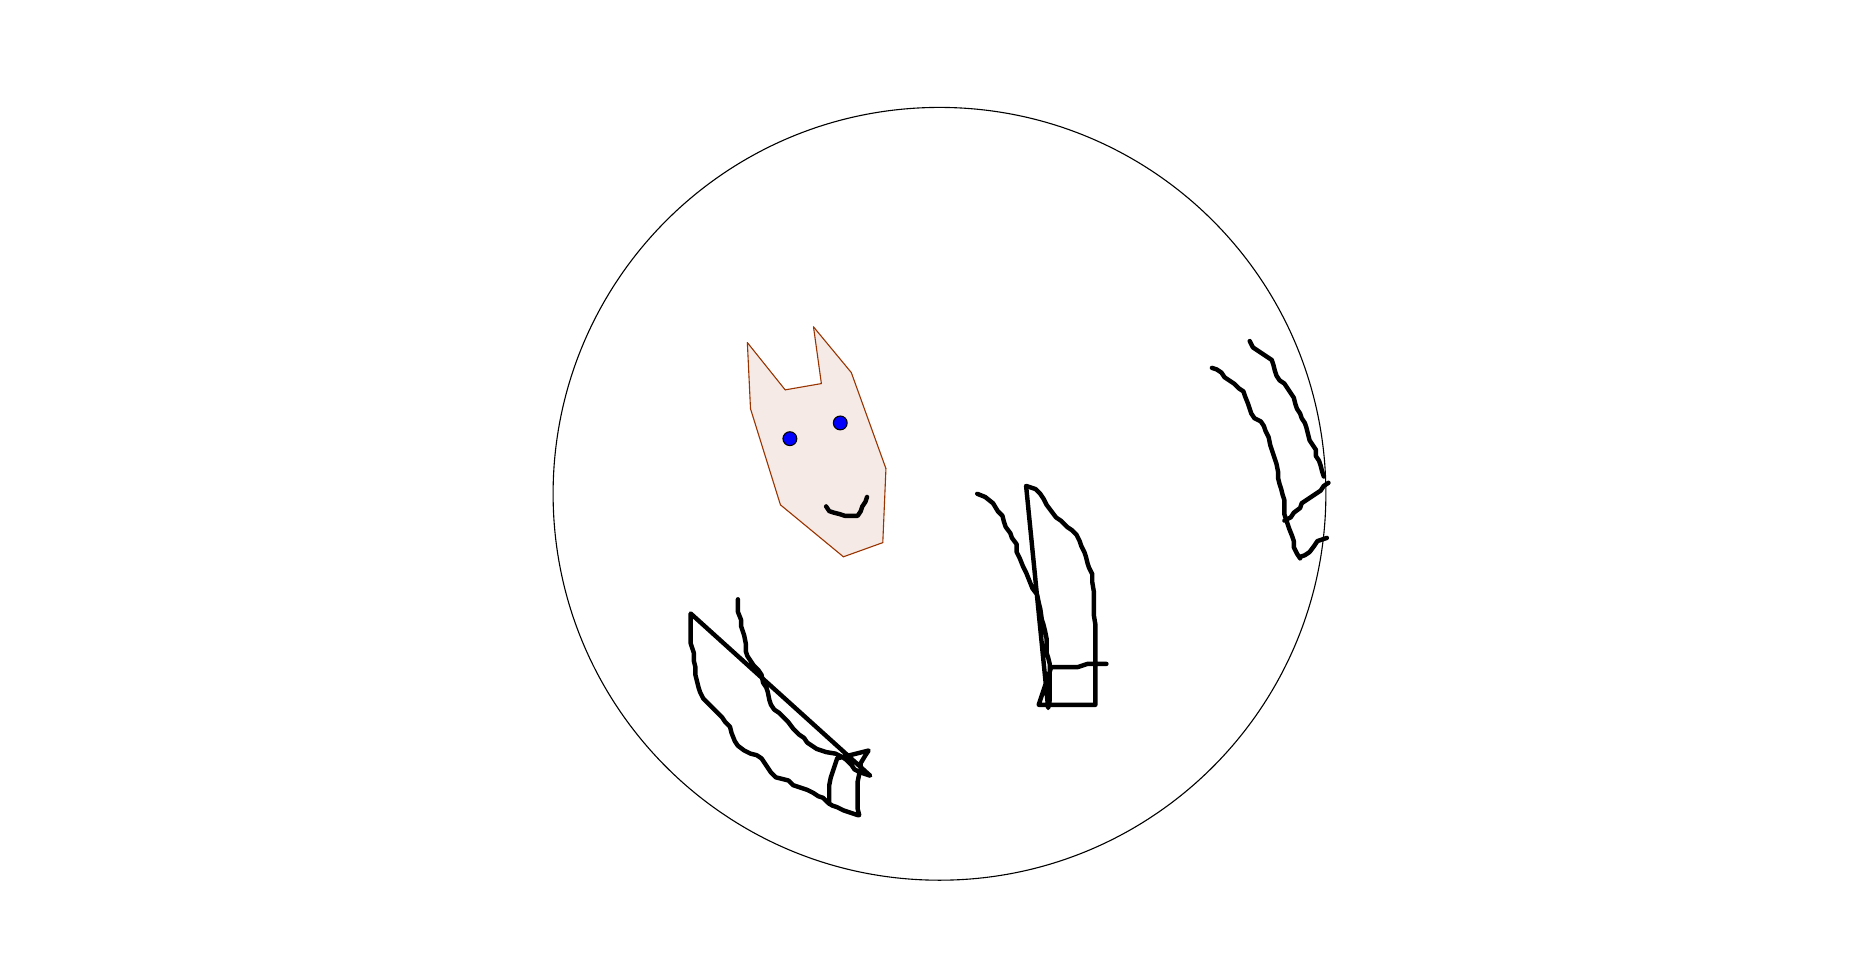
\begin{tikzpicture}[line cap=round,line join=round,>=triangle 45,x=1.0cm,y=1.0cm]
\clip(-3.36,0.08) rectangle (19.64,11.72);
\fill[color=zzttqq,fill=zzttqq,fill opacity=0.10000000149011612] (5.82,6.88) -- (6.2,5.66) -- (7.,5.) -- (7.5,5.18) -- (7.54,6.12) -- (7.1,7.34) -- (6.62,7.92) -- (6.72,7.2) -- (6.26,7.12) -- (5.78,7.72) -- cycle;
\draw(8.22,5.8) circle (4.90717841534216cm);
\draw [color=zzttqq] (5.82,6.88)-- (6.2,5.66);
\draw [color=zzttqq] (6.2,5.66)-- (7.,5.);
\draw [color=zzttqq] (7.,5.)-- (7.5,5.18);
\draw [color=zzttqq] (7.5,5.18)-- (7.54,6.12);
\draw [color=zzttqq] (7.54,6.12)-- (7.1,7.34);
\draw [color=zzttqq] (7.1,7.34)-- (6.62,7.92);
\draw [color=zzttqq] (6.62,7.92)-- (6.72,7.2);
\draw [color=zzttqq] (6.72,7.2)-- (6.26,7.12);
\draw [color=zzttqq] (6.26,7.12)-- (5.78,7.72);
\draw [color=zzttqq] (5.78,7.72)-- (5.82,6.88);
\draw [line width=1.6pt] (8.7,5.8)-- (8.7,5.8)-- (8.7,5.8)-- (8.8,5.76)-- (8.9,5.68)-- (8.96,5.58)-- (9.02,5.52)-- (9.04,5.44)-- (9.06,5.38)-- (9.12,5.3)-- (9.14,5.24)-- (9.2,5.16)-- (9.2,5.06)-- (9.24,4.98)-- (9.28,4.88)-- (9.32,4.8)-- (9.36,4.7)-- (9.4,4.6)-- (9.46,4.52)-- (9.48,4.42)-- (9.5,4.34)-- (9.52,4.2)-- (9.54,4.14)-- (9.56,4.06)-- (9.58,3.96)-- (9.58,3.88)-- (9.58,3.78)-- (9.6,3.72)-- (9.62,3.64)-- (9.62,3.56)-- (9.62,3.46)-- (9.62,3.36)-- (9.62,3.28)-- (9.62,3.18)-- (9.6,3.08)-- (9.32,5.9)-- (9.32,5.9)-- (9.32,5.9)-- (9.32,5.9)-- (9.38,5.88)-- (9.44,5.86)-- (9.5,5.8)-- (9.54,5.74)-- (9.58,5.66)-- (9.64,5.58)-- (9.7,5.5)-- (9.76,5.46)-- (9.84,5.38)-- (9.9,5.34)-- (9.96,5.28)-- (10.,5.2)-- (10.02,5.14)-- (10.06,5.06)-- (10.08,5.)-- (10.1,4.92)-- (10.12,4.86)-- (10.16,4.78)-- (10.16,4.68)-- (10.18,4.56)-- (10.18,4.44)-- (10.18,4.34)-- (10.18,4.26)-- (10.2,4.14)-- (10.2,3.98)-- (10.2,3.88)-- (10.2,3.76)-- (10.2,3.62)-- (10.2,3.5)-- (10.2,3.4)-- (10.2,3.32)-- (10.2,3.24)-- (10.2,3.16)-- (10.2,3.16)-- (10.2,3.12)-- (10.2,3.12)-- (10.2,3.12)-- (10.08,3.12)-- (10.,3.12)-- (9.9,3.12)-- (9.82,3.12)-- (9.72,3.12)-- (9.64,3.12)-- (9.56,3.12)-- (9.48,3.12)-- (9.48,3.12)-- (9.64,3.6)-- (9.64,3.6)-- (9.64,3.6)-- (9.72,3.6)-- (9.8,3.6)-- (9.88,3.6)-- (9.98,3.6)-- (10.04,3.62)-- (10.1,3.64)-- (10.18,3.64)-- (10.26,3.64)-- (10.34,3.64);
\draw [line width=1.6pt] (5.66,4.46)-- (5.66,4.46)-- (5.66,4.46)-- (5.66,4.38)-- (5.66,4.3)-- (5.7,4.2)-- (5.7,4.12)-- (5.74,4.)-- (5.76,3.9)-- (5.76,3.8)-- (5.78,3.74)-- (5.82,3.68)-- (5.86,3.62)-- (5.92,3.56)-- (5.96,3.5)-- (5.98,3.4)-- (6.02,3.34)-- (6.04,3.28)-- (6.06,3.18)-- (6.08,3.12)-- (6.12,3.06)-- (6.18,3.02)-- (6.24,2.96)-- (6.3,2.9)-- (6.36,2.82)-- (6.44,2.74)-- (6.5,2.7)-- (6.54,2.64)-- (6.6,2.6)-- (6.66,2.56)-- (6.72,2.54)-- (6.78,2.52)-- (6.9,2.5)-- (6.98,2.46)-- (7.04,2.42)-- (7.1,2.36)-- (7.14,2.3)-- (7.22,2.26)-- (7.28,2.24)-- (7.34,2.22)-- (7.34,2.22)-- (5.06,4.28)-- (5.06,4.28)-- (5.06,4.28)-- (5.06,4.2)-- (5.06,4.1)-- (5.06,4.)-- (5.06,3.9)-- (5.08,3.84)-- (5.1,3.78)-- (5.1,3.68)-- (5.12,3.6)-- (5.12,3.5)-- (5.14,3.42)-- (5.16,3.34)-- (5.18,3.28)-- (5.22,3.2)-- (5.28,3.14)-- (5.34,3.08)-- (5.4,3.02)-- (5.46,2.96)-- (5.5,2.9)-- (5.56,2.84)-- (5.58,2.76)-- (5.62,2.66)-- (5.66,2.6)-- (5.74,2.54)-- (5.82,2.5)-- (5.9,2.48)-- (5.96,2.44)-- (6.,2.38)-- (6.04,2.32)-- (6.08,2.26)-- (6.14,2.2)-- (6.22,2.18)-- (6.3,2.16)-- (6.36,2.1)-- (6.42,2.08)-- (6.48,2.06)-- (6.54,2.04)-- (6.62,2.)-- (6.68,1.96)-- (6.74,1.94)-- (6.8,1.88)-- (6.86,1.84)-- (6.92,1.82)-- (7.,1.78)-- (7.06,1.76)-- (7.12,1.74)-- (7.18,1.72)-- (7.18,1.72)-- (7.2,1.72)-- (7.2,1.72)-- (7.2,1.72)-- (7.18,1.8)-- (7.18,1.88)-- (7.18,1.98)-- (7.18,2.06)-- (7.18,2.14)-- (7.2,2.24)-- (7.22,2.3)-- (7.22,2.38)-- (7.28,2.48)-- (7.32,2.54)-- (7.32,2.54)-- (6.92,2.44)-- (6.92,2.44)-- (6.92,2.44)-- (6.88,2.32)-- (6.84,2.2)-- (6.82,2.1)-- (6.82,2.02)-- (6.82,1.94)-- (6.82,1.86);
\draw [line width=1.6pt] (6.78,5.64)-- (6.78,5.64)-- (6.78,5.64)-- (6.82,5.58)-- (6.88,5.56)-- (6.96,5.54)-- (7.02,5.52)-- (7.1,5.52)-- (7.18,5.52)-- (7.22,5.58)-- (7.24,5.64)-- (7.28,5.7)-- (7.3,5.76);
\draw [line width=1.6pt] (11.68,7.4)-- (11.68,7.4)-- (11.68,7.4)-- (11.74,7.38)-- (11.8,7.34)-- (11.84,7.28)-- (11.9,7.24)-- (11.96,7.2)-- (12.02,7.14)-- (12.08,7.1)-- (12.1,7.04)-- (12.14,6.94)-- (12.16,6.88)-- (12.18,6.82)-- (12.22,6.76)-- (12.3,6.72)-- (12.34,6.66)-- (12.36,6.6)-- (12.4,6.52)-- (12.42,6.42)-- (12.44,6.36)-- (12.46,6.3)-- (12.48,6.24)-- (12.5,6.18)-- (12.52,6.08)-- (12.52,6.)-- (12.54,5.92)-- (12.56,5.86)-- (12.58,5.78)-- (12.6,5.72)-- (12.6,5.64)-- (12.6,5.54)-- (12.62,5.48)-- (12.64,5.42)-- (12.66,5.36)-- (12.7,5.26)-- (12.72,5.2)-- (12.72,5.12)-- (12.76,5.04)-- (12.8,4.98);
\draw [line width=1.6pt] (12.16,7.74)-- (12.16,7.74)-- (12.16,7.74)-- (12.2,7.66)-- (12.26,7.62)-- (12.32,7.58)-- (12.38,7.54)-- (12.44,7.5)-- (12.46,7.44)-- (12.48,7.36)-- (12.5,7.3)-- (12.54,7.24)-- (12.6,7.2)-- (12.64,7.14)-- (12.68,7.08)-- (12.72,7.02)-- (12.74,6.94)-- (12.76,6.88)-- (12.8,6.82)-- (12.82,6.76)-- (12.86,6.7)-- (12.88,6.64)-- (12.9,6.56)-- (12.92,6.48)-- (12.96,6.42)-- (13.,6.36)-- (13.,6.28)-- (13.04,6.22)-- (13.06,6.16)-- (13.08,6.08)-- (13.1,6.02);
\draw [line width=1.6pt] (12.8,5.)-- (12.8,5.)-- (12.8,5.)-- (12.86,5.02)-- (12.92,5.06)-- (12.98,5.14)-- (13.02,5.2)-- (13.08,5.22)-- (13.14,5.24);
\draw [line width=1.6pt] (12.6,5.46)-- (12.6,5.46)-- (12.6,5.46)-- (12.68,5.5)-- (12.72,5.56)-- (12.8,5.62)-- (12.82,5.68)-- (12.88,5.72)-- (12.94,5.76)-- (13.,5.8)-- (13.06,5.84)-- (13.1,5.9)-- (13.16,5.94);
\begin{scriptsize}
\draw [fill=qqqqff] (6.32,6.5) circle (2.5pt);
\draw [fill=qqqqff] (6.96,6.7) circle (2.5pt);
\end{scriptsize}
\end{tikzpicture}
}


     % Автор: Кунакбаева Камила

% Автор: Маликова Ольга

\definecolor{ffffff}{rgb}{1.,1.,1.}
\definecolor{ffdxqq}{rgb}{1.,0.8431372549019608,0.}

\newenvironment{nkorob}
    {\renewcommand{\arraystretch}{1}
    \begin{center}
    \begin{tabular}{|p{0.5\textwidth}|}
    \hline \vspace{1pt} 
    }{ 
    \vspace{5pt} \\ \hline 
    \end{tabular} 
    \end{center}
    }
\newcommand{\nbillsay}[2]{
\begin{nkorob}
#1
\end{nkorob}

\begin{tikzpicture}[scale=#2,line cap=round,line join=round,>=triangle 45,x=0.8177493455226243cm,y=0.8547418890802324cm]
\fill[color=ffdxqq,fill=ffdxqq,fill opacity=1.0] (5.,5.) -- (3.5,1.98) -- (6.52,1.98) -- cycle;
\fill[fill=black,fill opacity=1.0] (4.440312912104037,2.659499439265859) -- (4.440312912104037,2.3099108932265446) -- (5.191928286088566,2.528403734501116) -- cycle;
\fill[fill=black,fill opacity=1.0] (4.789901458143351,2.5021845935481672) -- (5.524037404825916,2.711937721171756) -- (5.54151683212788,2.32739032052851) -- cycle;
\fill[fill=black,fill opacity=1.0] (4.6147293124731465,5.293143013725243) -- (4.6147293124731465,5.036085922223045) -- (5.346327063253401,5.023295824039814) -- (5.337426967126186,5.281398611729002) -- cycle;
\fill[fill=black,fill opacity=1.0] (4.839021584002231,5.904405340633938) -- (4.901322256892725,5.174597458202441) -- (5.061523987182569,5.183497554329654) -- (5.132724756200276,5.913305436761151) -- cycle;
\draw [color=ffdxqq] (5.,5.)-- (3.5,1.98);
\draw [rotate around={0.:(5.,3.48)}] (5.,3.48) ellipse (0.4857640546613854cm and 0.27413962542252507cm);
\draw [rotate around={0.:(5.,3.48)},color=ffffff,fill=ffffff,fill opacity=1.0] (5.,3.48) ellipse (0.4857640546613854cm and 0.27413962542252507cm);
\draw (4.440312912104037,2.659499439265859)-- (4.440312912104037,2.3099108932265446);
\draw (4.440312912104037,2.3099108932265446)-- (5.191928286088566,2.528403734501116);
\draw (5.191928286088566,2.528403734501116)-- (4.440312912104037,2.659499439265859);
\draw (4.789901458143351,2.5021845935481672)-- (5.524037404825916,2.711937721171756);
\draw (5.524037404825916,2.711937721171756)-- (5.54151683212788,2.32739032052851);
\draw (5.54151683212788,2.32739032052851)-- (4.789901458143351,2.5021845935481672);
\draw (4.794836142917474,3.780991442527641)-- (4.702418183898973,3.9635573421136203);
\draw (4.978809382274053,3.8274249342152835)-- (4.970744820023095,4.009229961028364);
\draw (5.150375800444393,3.808898576330301)-- (5.221944224054187,3.9921027289353352);
\draw (4.736467691529514,2.9810823585005783)-- (4.808036115139318,3.1642865111056055);
\draw [line width=1.2pt] (5.015918385142284,2.971063329563836)-- (5.007853822891325,3.1528683563769193);
\draw [line width=1.2pt] (5.254416870747083,2.987429688883977)-- (5.161998911728586,3.1699955884699484);
\draw (4.6147293124731465,5.293143013725243)-- (4.6147293124731465,5.036085922223045);
\draw (4.6147293124731465,5.036085922223045)-- (5.346327063253401,5.023295824039814);
\draw (5.346327063253401,5.023295824039814)-- (5.337426967126186,5.281398611729002);
\draw (5.337426967126186,5.281398611729002)-- (4.6147293124731465,5.293143013725243);
\draw (4.839021584002231,5.904405340633938)-- (4.901322256892725,5.174597458202441);
\draw (4.901322256892725,5.174597458202441)-- (5.061523987182569,5.183497554329654);
\draw (5.061523987182569,5.183497554329654)-- (5.132724756200276,5.913305436761151);
\draw (5.132724756200276,5.913305436761151)-- (4.839021584002231,5.904405340633938);
\draw [line width=1.6pt] (3.2158610934714873,3.122323687751398)-- (4.05106119768379,3.1142149488755506);
\draw [line width=2.pt] (5.960669202945901,3.0898887322480078)-- (6.7958693071582035,3.0817799933721606);
\draw [line width=2.pt] (3.2158610934714873,3.122323687751398)-- (2.9979803020821847,3.135959019861279);
\draw [line width=2.pt] (3.2158610934714873,3.122323687751398)-- (3.0791761824154027,2.9707544497314324);
\draw [line width=1.2pt] (6.950214461233794,3.0729774323863963)-- (6.7323336698444916,3.0866127644962775);
\draw [line width=1.6pt] (6.879185601996351,2.897622756187366)-- (6.7540571038629,3.079371619823475);
\draw [line width=1.2pt] (6.897983159591788,3.2526642918618487)-- (6.761298248535703,3.1010950538418833);
\draw [rotate around={-2.1271774882113834:(3.2134475402921185,3.124100864581607)},fill=black,fill opacity=1.0] (3.2134475402921185,3.124100864581607) ellipse (0.07464387565286307cm and 0.055656655159166346cm);
\draw [rotate around={-2.1271774882113688:(6.783324310765273,3.08794169866216)},fill=black,fill opacity=1.0] (6.783324310765273,3.08794169866216) ellipse (0.074643875652832cm and 0.05565665515914107cm);
\draw [rotate around={-87.43622978853486:(4.991645653927142,3.495593119750347)},fill=black,fill opacity=1.0] (4.991645653927142,3.495593119750347) ellipse (0.2311032663156497cm and 0.136710184251997cm);
\draw [line width=1.6pt] (3.1823709110106124,3.1533457427204454)-- (3.0572424128771614,3.335094606356554);
\draw [line width=2.pt] (4.686348292288832,1.9817608220216265)-- (4.20913420601832,1.297062350416114);
\draw [line width=2.pt] (5.336691780588076,1.970216394104754)-- (5.7858550793476144,1.273007691552639);
\draw [line width=2.pt] (5.7858550793476144,1.273007691552639)-- (5.430546798239323,0.7501011646385526);
\draw [line width=1.6pt] (4.20913420601832,1.297062350416114)-- (4.632779148203724,0.8171404629608713);
\draw [line width=5.2pt] (4.572443779713636,0.7098775856451613)-- (4.7668577448483616,0.9780347789344364);
\draw [line width=5.2pt] (5.4975860965616405,0.6361343574906106)-- (5.323283920923611,0.9244033402765813);
\draw(5.958929987043349,4.220908920040284) ellipse (0.13785013631684354cm and 0.1440860657003932cm);
\draw(6.991404759166196,5.097852672629884) ellipse (0.12289296225648996cm and 0.12845227365684486cm);
\draw(7.603360130208264,6.576520496453611) ellipse (0.12289296225648996cm and 0.12845227365684486cm);
\end{tikzpicture}}




\begin{document} 


\section{Применение: книжка для школьников?} 


Сегодня мы посвятим свое время лемме Ферма. Для тех, кто не в теме --- не той теореме, от которой люди сходят с ума(Перельман!) Нет, ма, --- формулировка леммы проста на удивление. Пусть функция имеет во внутренней точке области определения.

\begin{wrapfigure}{r}{0.3333\linewidth}
   \nbillsay{Запомните! Если функция непрерывна на    отрезке, то она равномерно непрерывна на нём!}{0.7}
 \caption{Мудрые советы от Билла} 
\end{wrapfigure}


Локальный экстремум --- минимум/максимум --- это неважно. И функция дифференцируема в этой точке, то скажем резко, дружно и слаженно: производная этой функции в точке экстремума будет нулю равна. Доказательство лучше молодого вина, во втором куплете представлено.

Знаешь ты, знаю я, знают он и она,
Знает целая страна.Производная в экстремуме нулю равна,
Нанананана, Нанананана.

Доказательство очень логично --- это вам не гражданское право: Производная есть? отлично --- возьмем как предел слева и справа. Если экстремум --- минимум, то производная слева всяко не больше нуля, ведь дельта игрек и дельта икс разного знака.Вот собака! Ведь справа этот же самый предел не смог бы стать меньше нуля, даже если б захотел: дельта игрек и дельта икс положительны оба. Дальше последний логический гвоздь в крышку гроба непонимания. Слева производная не больше нуля, справа не меньше. Внимание! Значит производная равна нулю, прям как в 39ом Польша! Все много проще, чем представлялось, мы в конце рассуждения, где все, что нам осталось, --- это написать ч.т.д.




\newpage

\section{Тоторо номер 1} 


\begin{pleasesay}{Тоторо --- хранитель леса, большое мохнатое существо серого цвета.}
\end{pleasesay}

\begin{pleasesay}{Тоторо --- хранитель леса, большое мохнатое существо серого цвета. Тоторо --- хранитель леса, большое мохнатое существо серого цвета. Тоторо --- хранитель леса, большое мохнатое существо серого цвета. Тоторо --- хранитель леса, большое мохнатое существо серого цвета.}
\end{pleasesay}


\newpage 

\section{Билл} 

\billsay{Remember! Reality is an illusion, the Universe is an hologram. Buy gold. Bye! Remember! Reality is an illusion, the Universe is an hologram. Buy gold. Bye! Remember! Reality is an illusion, the Universe is an hologram. Buy gold. Bye! Remember! Reality is an illusion, the Universe is an hologram. Buy gold. Bye!}

%Билл в Билле! 
\billsay{\billsay{Remember!}}

\newpage

\section{Тоторо номер 2} 

\begin{center}
\begin{totoro}
Я полупингвин - полумышь, хотя должен быть Тоторо.\\
Но я не виноват, это просто кто-то плохо рисует!\\
В geogebra у меня хоть глазные яблоки были, а тут совсем печалька!
И ещё у меня есть третий глаз для закрепления всей красоты.
\end{totoro}
\end{center}



\newpage 


\section{Кот} 

\begin{kot}
{Hello!}
\end{kot}


\newpage 

\section{Пеппа} 

\begin{peppa}
	Свинка Пеппа пам-пара-рам-рам-пам-парара-рам-пам
\end{peppa}


\newpage

\section{Корова} 

% Обратить внимание на сдвиг. Убрать clip.
\cowsay{Hello! I'm a bit ugly talking cow:)Hello! I'm a bit ugly talking cow:)  Hello! I'm a bit ugly talking cow:)  Hello! I'm a bit ugly talking cow:)  }



\newpage

\begin{spherkon}
Я сферический конь в вакууме!
\end{spherkon}

\newpage

\section{Модернизация Билла} 

\nbillsay{Remember! Reality is an illusion, the Universe is an hologram. Buy gold. Bye! Remember! Reality is an illusion, the Universe is an hologram. Buy gold. Bye! Remember! Reality is an illusion, the Universe is an hologram. Buy gold. Bye! Remember! Reality is an illusion, the Universe is an hologram. Buy gold. Bye!}{5}


\end{document}


